\section{Specimen \circled{1} : Michael-Scott queue}

% ---------------------------------------------------------

\begin{frame}{Original article (1996)}
\centering
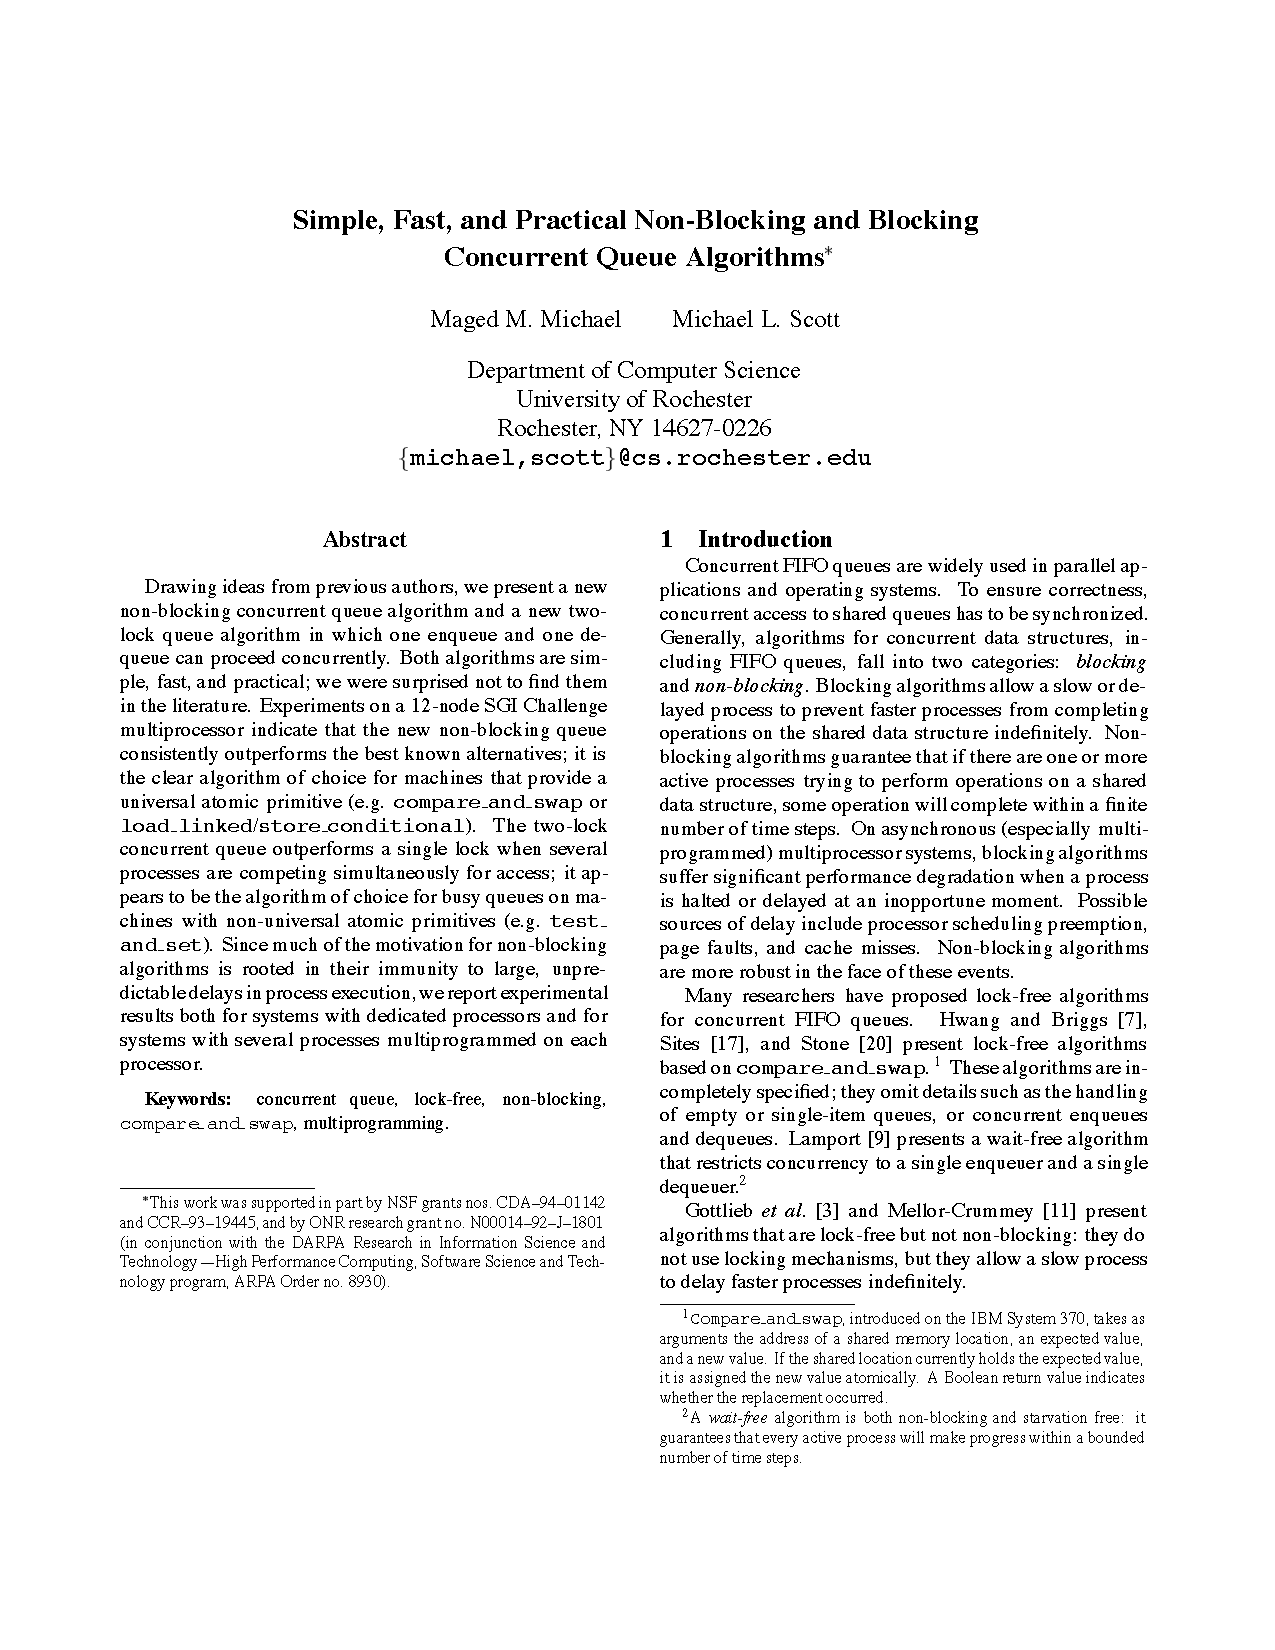
\includegraphics[scale=0.5]{images/michael_scott_1996.pdf}
\end{frame}

% ---------------------------------------------------------

\begin{frame}{Basic implementation}
TODO
\end{frame}

% ---------------------------------------------------------

\begin{frame}[fragile]{Basic \OCaml~5 implementation}
\begin{minted}{ocaml}
type 'a node =
  | Nil
  | Next of 'a * 'a node Atomic.t

type 'a t = {
  front: 'a node Atomic.t Atomic.t ;
  back: 'a node Atomic.t Atomic.t ;
}
\end{minted}
\end{frame}

% ---------------------------------------------------------

\begin{frame}{Specification}
\large
\[
  \aspec{
    \mathcolor{cyan}{\mathrm{queue \mathhyphen inv}}\ t\ \iota
  }{
    \mathit{vs}
  }{
    \mathcolor{orange}{\mathrm{queue \mathhyphen model}}\ t\ \mathit{vs}
  }{
    \texttt{queue\_push}\ t\ v,\ \uparrow \iota
  }{
    \mathcolor{orange}{\mathrm{queue \mathhyphen model}}\ t\ (\mathit{vs} \mdoubleplus [v])
  }{
    \texttt{()}
  }{
    \iTrue
  }
\]
\vfill
\[
  \aspec{
    \mathcolor{cyan}{\mathrm{queue \mathhyphen inv}}\ t\ \iota
  }{
    \mathit{vs}
  }{
    \mathcolor{orange}{\mathrm{queue \mathhyphen model}}\ t\ \mathit{vs}
  }{
    \texttt{queue\_pop}\ t,\ \uparrow \iota
  }{
    \mathcolor{orange}{\mathrm{queue \mathhyphen model}}\ t\ (\mathrm{tail}\ \mathit{vs})
  }{
    \mathrm{head}\ \mathit{vs}
  }{
    \iTrue
  }
\]
\end{frame}

% ---------------------------------------------------------

\begin{frame}{Verification by Vindum \& Birkedal (2021)}
\centering
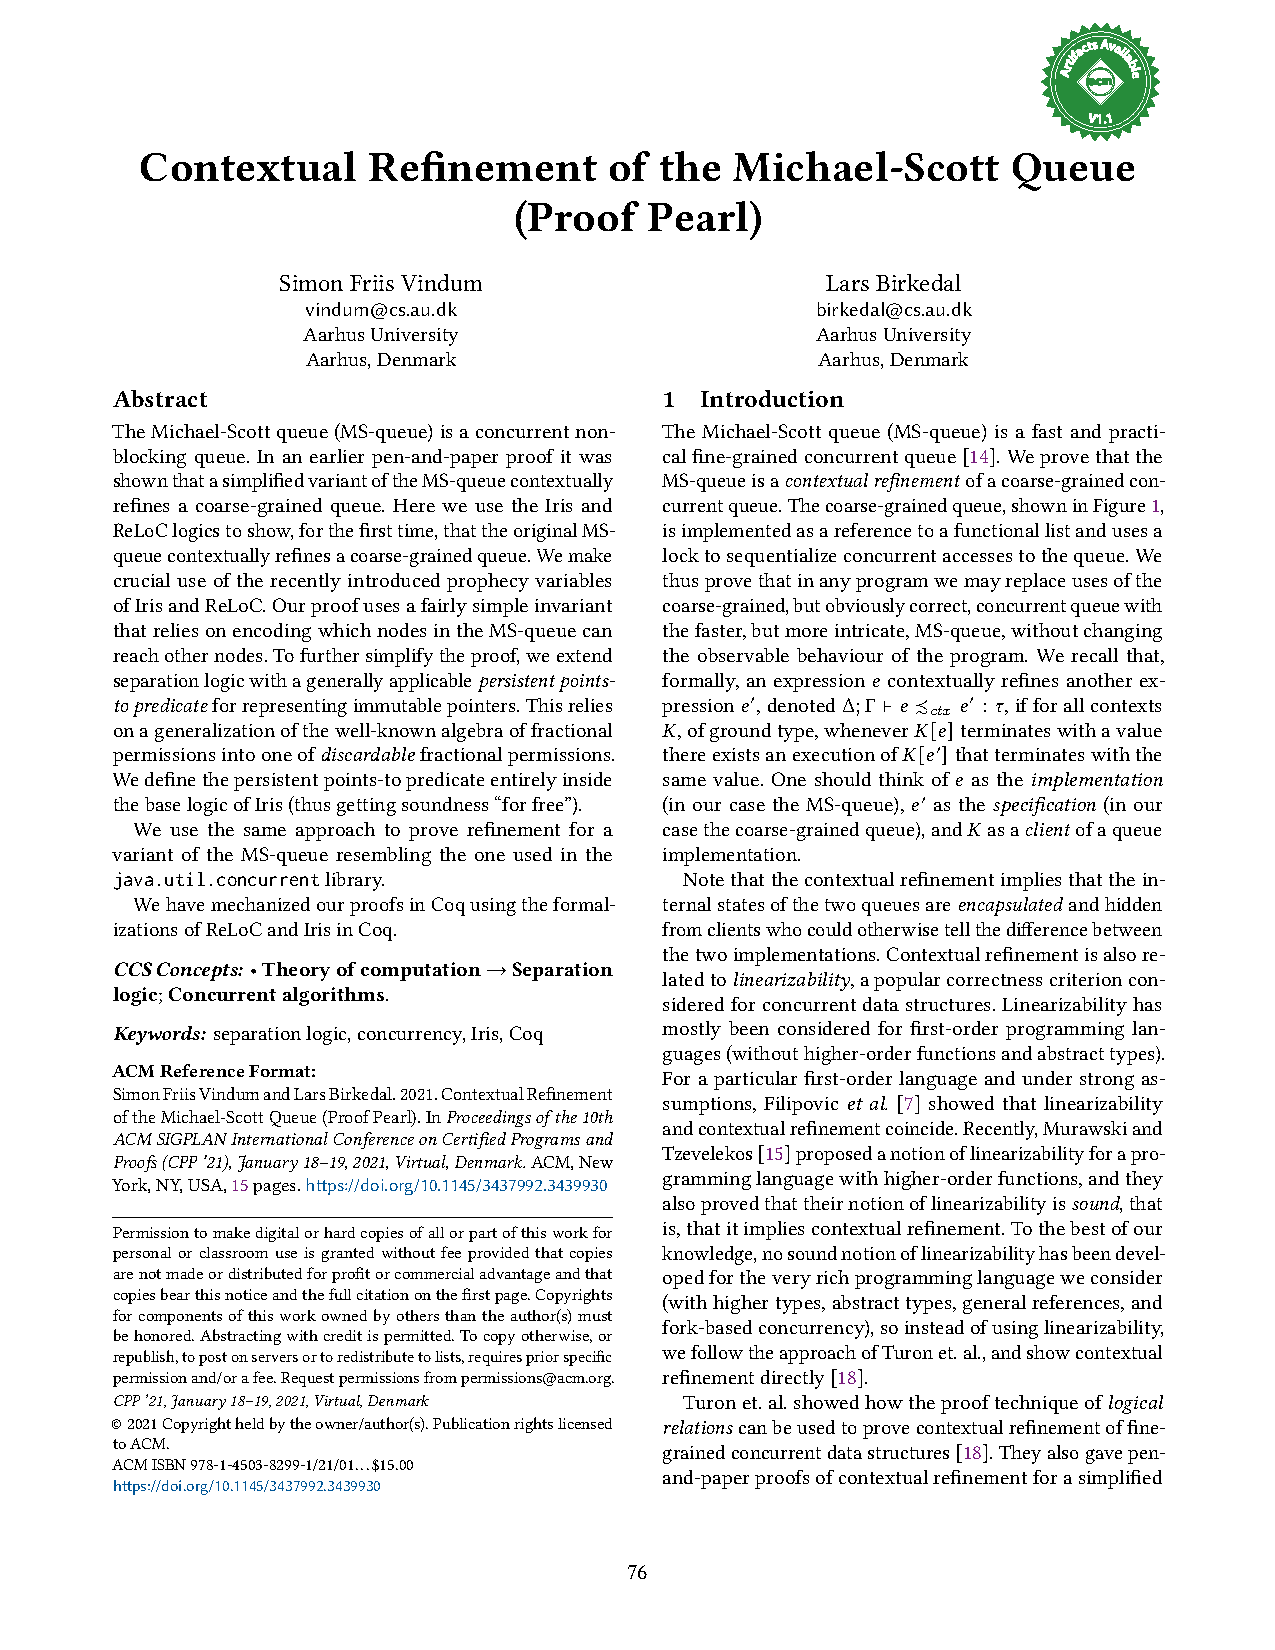
\includegraphics[scale=0.5]{images/vindum_birkedal_2021.pdf}
\end{frame}

% ---------------------------------------------------------

\begin{frame}{Optimized implementation}
TODO
\end{frame}

% ---------------------------------------------------------

\begin{frame}[fragile]{Optimized \OCaml~5 implementation --- first try}
\small
\begin{minted}{ocaml}
type ('a, _) t =
  | Nil : ('a, [> `Nil]) t
  | Next : {
      mutable next: ('a, [`Nil | `Next]) t ;
      mutable value: 'a ;
    } -> 
    ('a, [> `Next]) t

external as_atomic :
  ('a, [`Next]) t ->
  ('a, [`Nil | `Next]) t Atomic.t
= "%identity"

let push t v =
  ...
  if Atomic.compare_and_set (as_atomic back) Nil node
  then ...
  else ...
\end{minted}
\end{frame}

% ---------------------------------------------------------

\begin{frame}{A new hope}
\centering
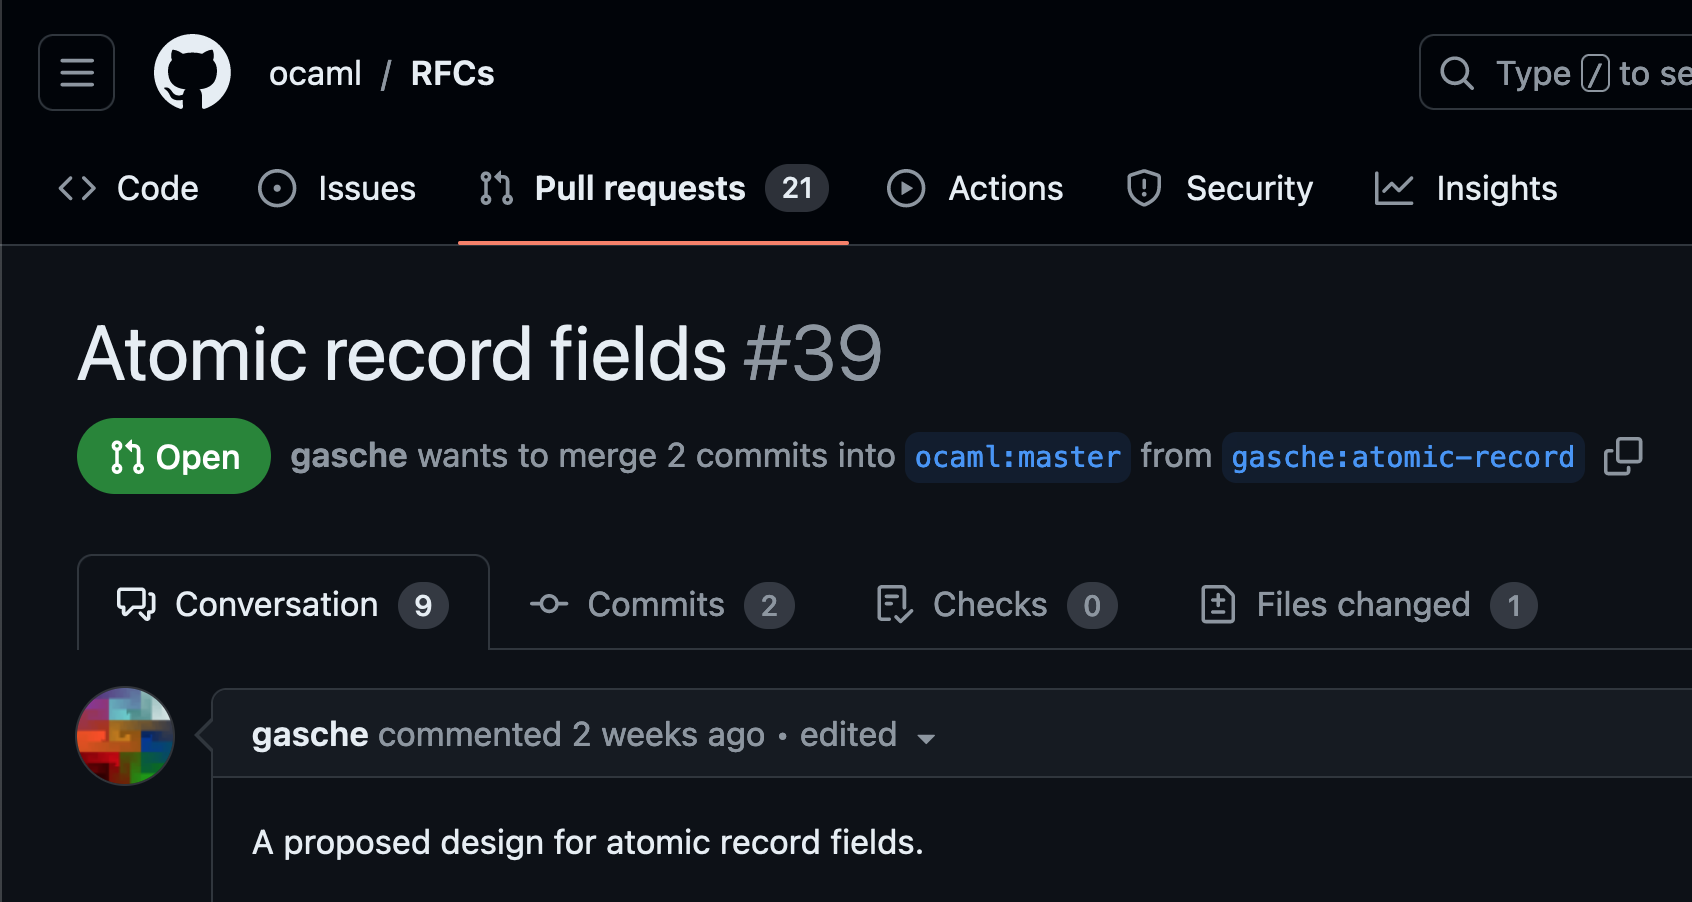
\includegraphics[scale=0.35]{images/rfc.png}
\vfill
(no modification of the \OCaml~5 memory model)
\end{frame}

% ---------------------------------------------------------

\begin{frame}[fragile]{Optimized \OCaml~5 implementation --- second try}
\begin{minted}{ocaml}
type 'a t =
  | Nil
  | Next of {
      mutable next: 'a t [@atomic] ;
      mutable value: 'a ;
    }

let push t v =
  ...
  if Atomic.Loc.compare_and_set
     [%atomic.field back.next]
     Nil node
  then ...
  else ...
\end{minted}
\end{frame}

% ---------------------------------------------------------

\begin{frame}{What about \texttt{is\_empty}?}
\large
\[
  \aspec{
    \mathcolor{cyan}{\mathrm{queue \mathhyphen inv}}\ t\ \iota
  }{
    \mathit{vs}
  }{
    \mathcolor{orange}{\mathrm{queue \mathhyphen model}}\ t\ \mathit{vs}
  }{
    \texttt{queue\_is\_empty}\ t,\ \uparrow \iota
  }{
    \mathcolor{orange}{\mathrm{queue \mathhyphen model}}\ t\ \mathit{vs}
  }{
    \mathit{vs} \stackrel{?}{=} \texttt{[]}
  }{
    \iTrue
  }
\]
\vfill
TODO
\end{frame}

% ---------------------------------------------------------

\begin{frame}{\Iris Invariant}
TODO
\end{frame}

% ---------------------------------------------------------

\begin{frame}{Space complexity}
\centering
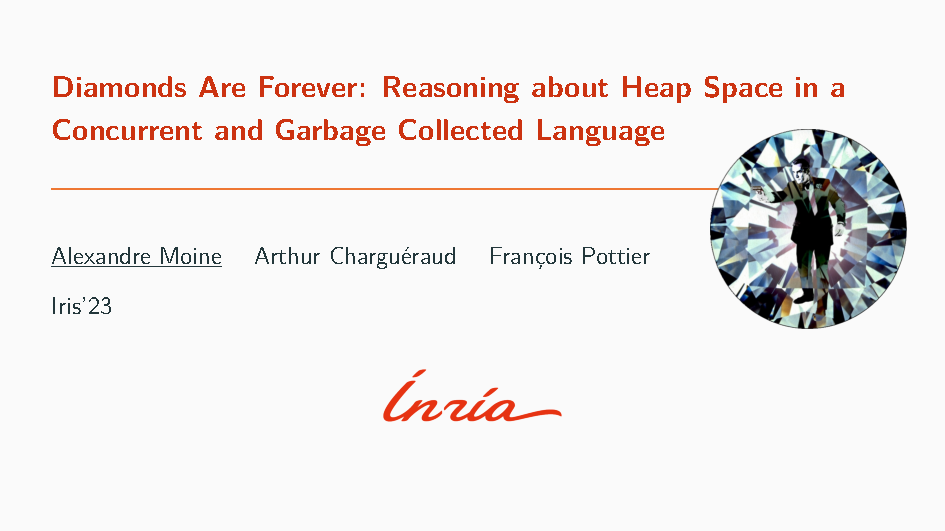
\includegraphics[scale=0.65]{images/moine_2023.pdf}
\end{frame}